\documentclass{beamer}

% Theme choices
\usetheme{Madrid}
\usecolortheme{dolphin}
\usefonttheme{professionalfonts}

\usepackage{svg}
\usepackage{minted}
\usepackage{xcolor}
\usepackage{adjustbox}


% Define colors for code highlighting
\definecolor{codebg}{rgb}{0.95,0.95,0.95}

% Minted settings
% Set the style for syntax highlighting
\usemintedstyle{friendly}


\newcommand{\motivationTitle}{How much sand is needed to fill the cave and its surroundings?}

% ----------------------------------------------------------------------------------------------------------------
% --- document ---------------------------------------------------------------------------------------------------
% ----------------------------------------------------------------------------------------------------------------

% Title page details
\title[Advent of Code 2022 Day 14]{Advent of Code 2022 Day 14}
\subtitle{Selected Fun Problems of the ACM Programming Contest}
\author{Simon Roller}
\institute{University of Tübingen}
\date{\today} % todo-----------------------------------------------------------------------------------------------

\begin{document}

% Title page
\begin{frame}
    \titlepage
\end{frame}

\section{Motivation}

\begin{frame}{Motivation}
    \motivationTitle
    \begin{figure}[H]
        \centering
        \includesvg[width=0.5\textwidth]{Images/AoC22_14_00.svg}
    \end{figure}
\end{frame}

\section{Problem Example}

\begin{frame}{Problem Example}
    \only<1>{
        \phantom{\motivationTitle}
        \begin{center}
            \includesvg[width=0.5\textwidth]{Images/AoC22_14_01.svg}
        \end{center}
    }
    \only<2>{
        \phantom{\motivationTitle}
        \begin{center}
            \includesvg[width=0.5\textwidth]{Images/AoC22_14_02.svg}
        \end{center}
    }
    \only<3>{
        \phantom{\motivationTitle}
        \begin{center}
            \includesvg[width=0.5\textwidth]{Images/AoC22_14_03.svg}
        \end{center}
    }
    \only<4>{
        \phantom{\motivationTitle}
        \begin{center}
            \includesvg[width=0.5\textwidth]{Images/AoC22_14_04.svg}
        \end{center}
    }
    \only<5>{
        \phantom{\motivationTitle}
        \begin{center}
            \includesvg[width=0.5\textwidth]{Images/AoC22_14_05.svg}
        \end{center}
    }
    \only<6>{
        \phantom{\motivationTitle}
        \begin{center}
            \includesvg[width=0.5\textwidth]{Images/AoC22_14_06.svg}
        \end{center}
    }
    \only<7>{
        \phantom{\motivationTitle}
        \begin{center}
            \includesvg[width=0.5\textwidth]{Images/AoC22_14_07.svg}
        \end{center}
    }
    \only<8>{
        \phantom{\motivationTitle}
        \begin{center}
            \includesvg[width=0.5\textwidth]{Images/AoC22_14_08.svg}
        \end{center}
    }
    \only<9>{
        \phantom{\motivationTitle}
        \begin{center}
            \includesvg[width=0.5\textwidth]{Images/AoC22_14_09.svg}
        \end{center}
    }
    \only<10>{
        \phantom{\motivationTitle}
        \begin{center}
            \includesvg[width=0.5\textwidth]{Images/AoC22_14_10.svg}
        \end{center}
    }
    \only<11>{
        \phantom{\motivationTitle}
        \begin{center}
            \includesvg[width=0.5\textwidth]{Images/AoC22_14_11.svg}
        \end{center}
    }
    \only<12>{
        \phantom{\motivationTitle}
        \begin{center}
            \includesvg[width=0.5\textwidth]{Images/AoC22_14_12.svg}
        \end{center}
    }
    \only<13>{
        \phantom{\motivationTitle}
        \begin{center}
            \includesvg[width=0.5\textwidth]{Images/AoC22_14_13.svg}
        \end{center}
    }
    \only<14>{
        \phantom{\motivationTitle}
        \begin{center}
            \includesvg[width=0.5\textwidth]{Images/AoC22_14_14.svg}
        \end{center}
    }
    \only<15>{
        \phantom{\motivationTitle}
        \begin{center}
            \includesvg[width=0.5\textwidth]{Images/AoC22_14_15.svg}
        \end{center}
    }
    \only<16>{
        \phantom{\motivationTitle}
        \begin{center}
            \includesvg[width=0.5\textwidth]{Images/AoC22_14_16.svg}
        \end{center}
    }
    \only<17>{
        \phantom{\motivationTitle}
        \begin{center}
            \includesvg[width=0.5\textwidth]{Images/AoC22_14_17.svg}
        \end{center}
    }
    \only<18>{
        \phantom{\motivationTitle}
        \begin{center}
            \includesvg[width=0.5\textwidth]{Images/AoC22_14_18.svg}
        \end{center}
    }
    \only<19>{
        \phantom{\motivationTitle}
        \begin{center}
            \includesvg[width=0.5\textwidth]{Images/AoC22_14_19.svg}
        \end{center}
    }
    \only<20>{
        \phantom{\motivationTitle}
        \begin{center}
            \includesvg[width=0.5\textwidth]{Images/AoC22_14_20.svg}
        \end{center}
    }
    \only<21>{
        \phantom{\motivationTitle}
        \begin{center}
            \includesvg[width=0.5\textwidth]{Images/AoC22_14_21.svg}
        \end{center}
    }
    \only<22>{
        \phantom{\motivationTitle}
        \begin{center}
            \includesvg[width=0.5\textwidth]{Images/AoC22_14_22.svg}
        \end{center}
    }
    \only<23>{
        \phantom{\motivationTitle}
        \begin{center}
            \includesvg[width=0.5\textwidth]{Images/AoC22_14_23.svg}
        \end{center}
    }
    \only<24>{
        \phantom{\motivationTitle}
        \begin{center}
            \includesvg[width=0.5\textwidth]{Images/AoC22_14_24.svg}
        \end{center}
    }
    \only<25>{
        \phantom{\motivationTitle}
        \begin{center}
            \includesvg[width=0.5\textwidth]{Images/AoC22_14_25.svg}
        \end{center}
    }
    \only<26>{
        \begin{center}
            \adjustbox{raise=0cm, margin=0 0 12.8 24}{\includesvg[width=0.5372\textwidth]{Images/AoC22_14_26.svg}}
        \end{center}
    }
\end{frame}

\section{Programming Language}

\begin{frame}{Programming Language}
    \begin{minipage}[c]{0.4\textwidth}
        \begin{itemize}
            \only{\item<1-> ease of use}
            \only{\item<2-> no runtime or memory constraints}
            \only{\item<3-> me being proficient in the language}
        \end{itemize}
    \end{minipage}%
    \begin{minipage}[c]{0.6\textwidth}
        \begin{figure}[H]
            \centering
            
\includegraphics[width=0.5\textwidth]{Images/python_logo.png}
        \end{figure}
    \end{minipage}
\end{frame}

\section{Input Details}

\begin{frame}[fragile]{Input Details}
    \begin{minted}[bgcolor=codebg, linenos, fontsize=\footnotesize]{python}
498,4 -> 498,6 -> 496,6
503,4 -> 502,4 -> 502,9 -> 494,9
    \end{minted}
    \pause
    \begin{minipage}[c]{0.4\textwidth}
        \begin{figure}[H]
            \centering
            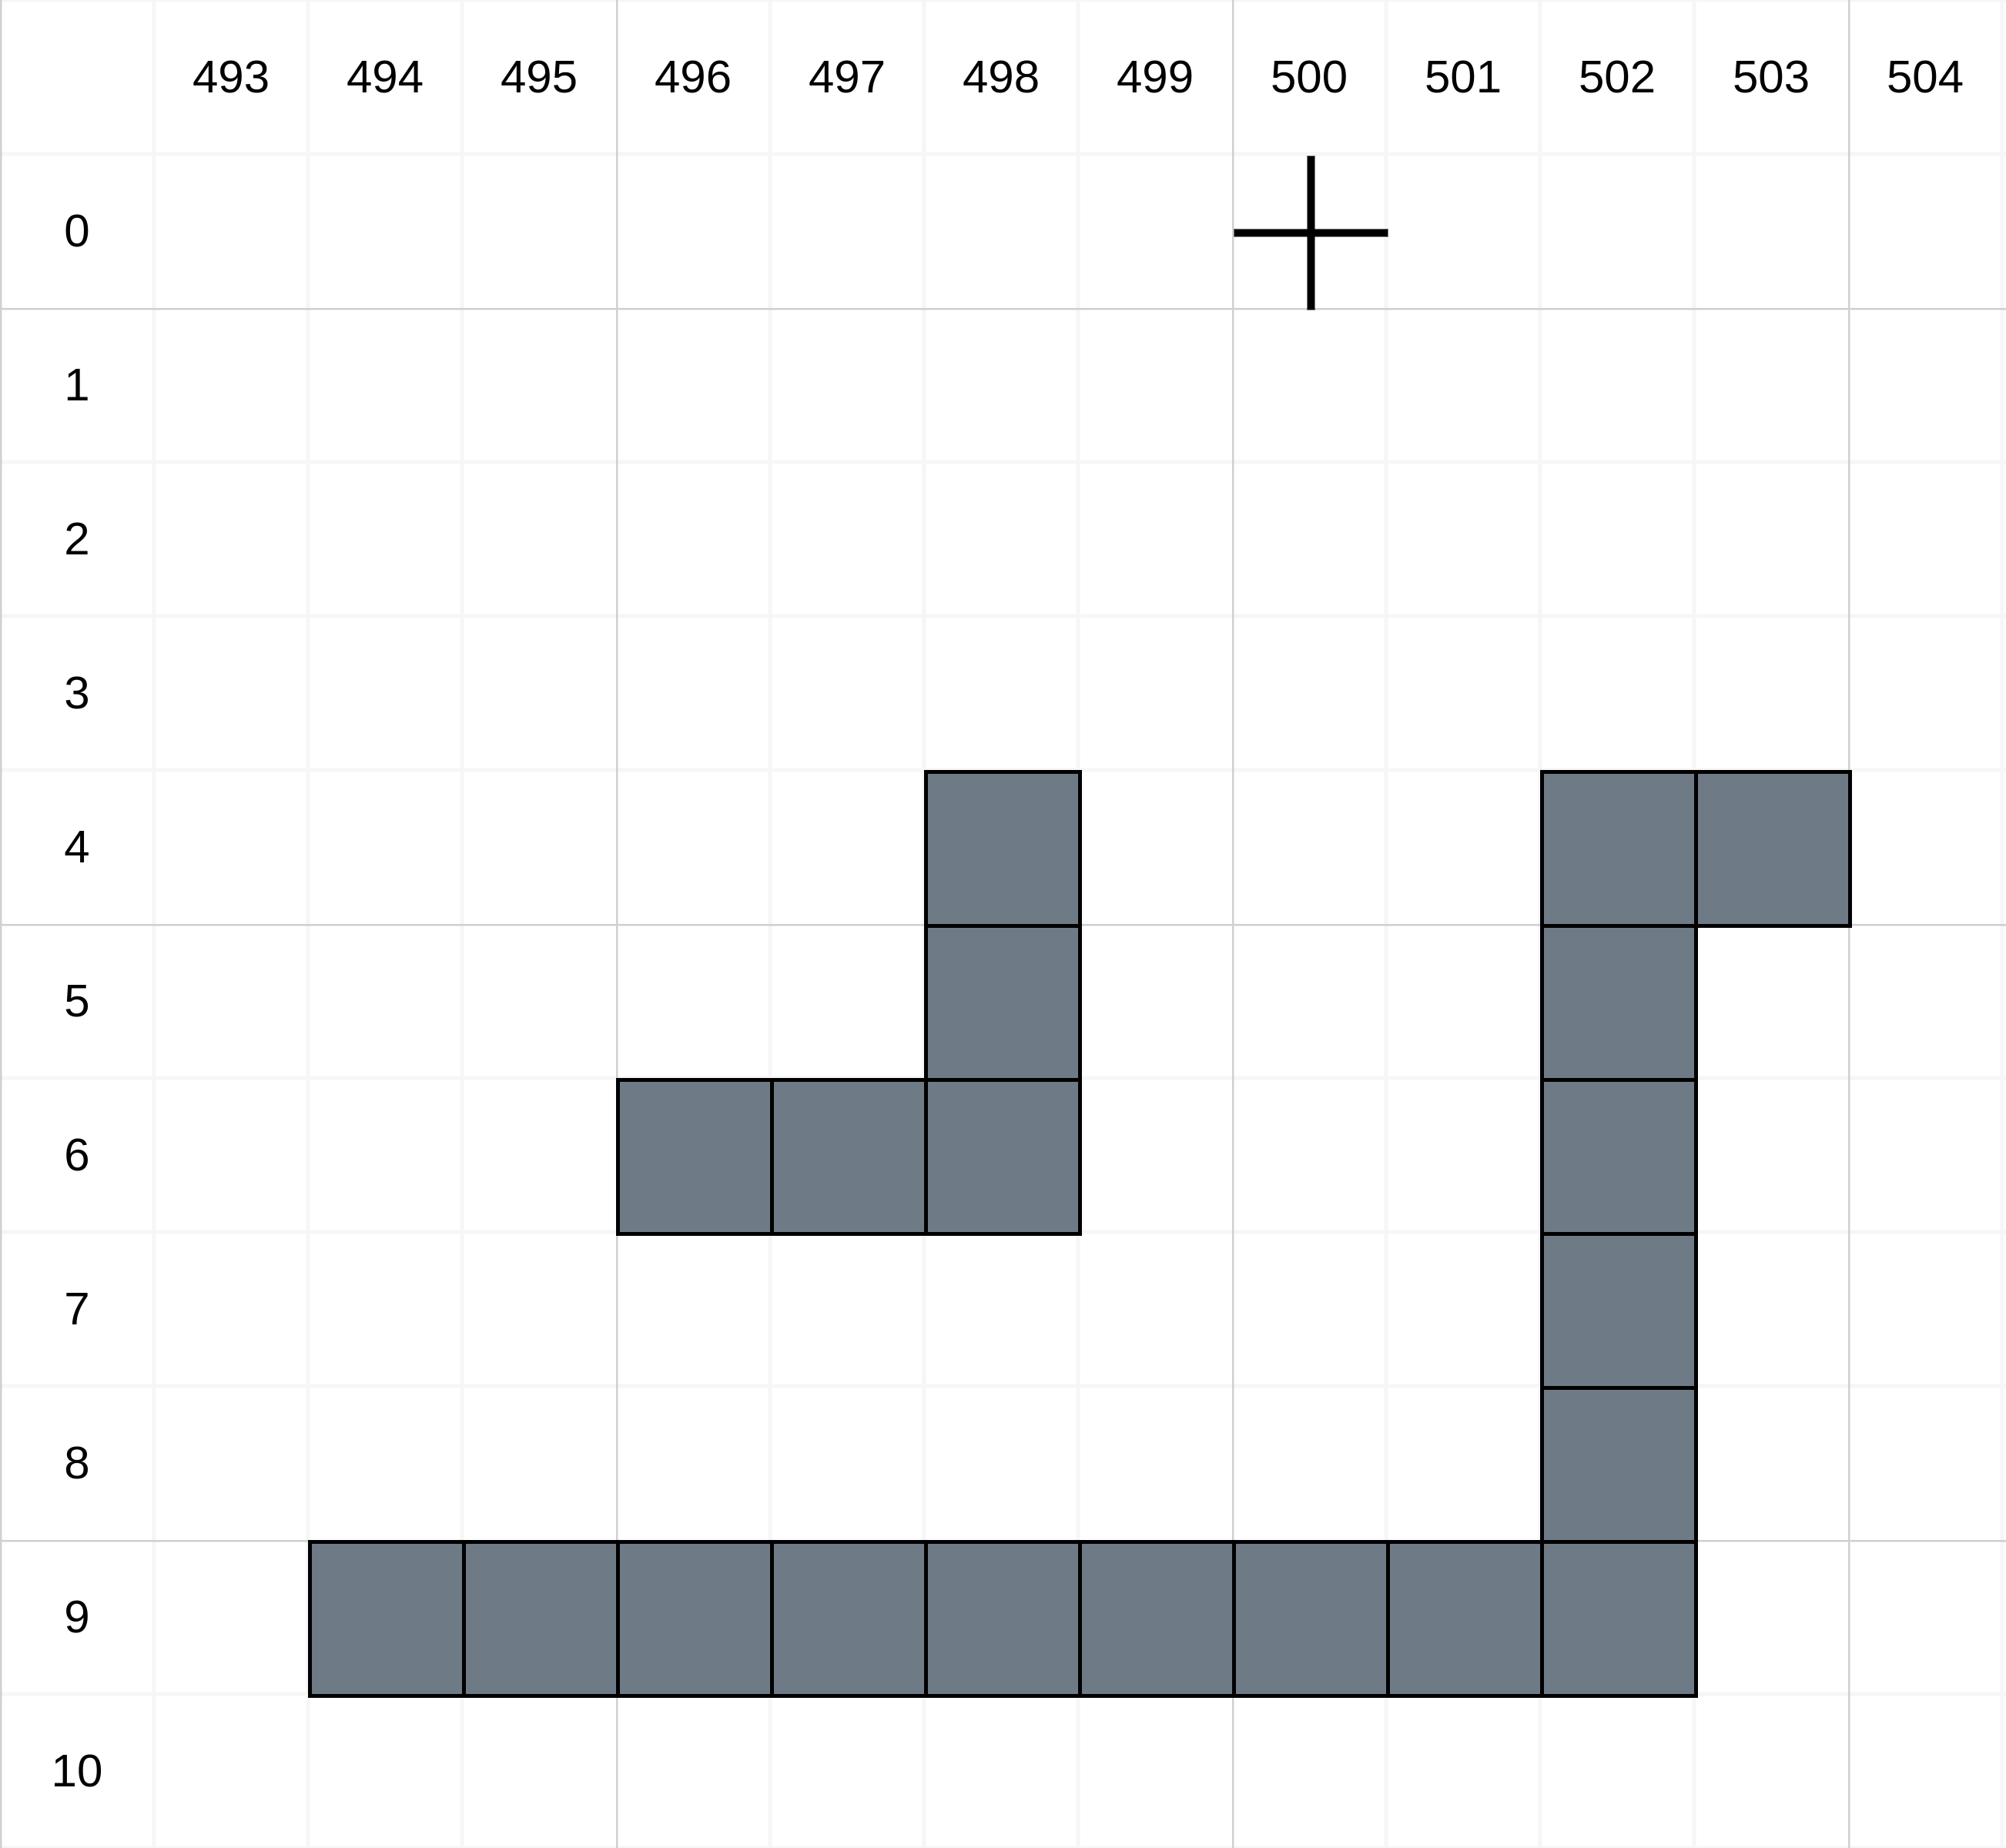
\includegraphics[width=0.8\textwidth]{Images/AoC22_14_00_grid.png}
        \end{figure}
    \end{minipage}%
    \begin{minipage}[c]{0.6\textwidth}
        \begin{figure}[H]
            \centering
            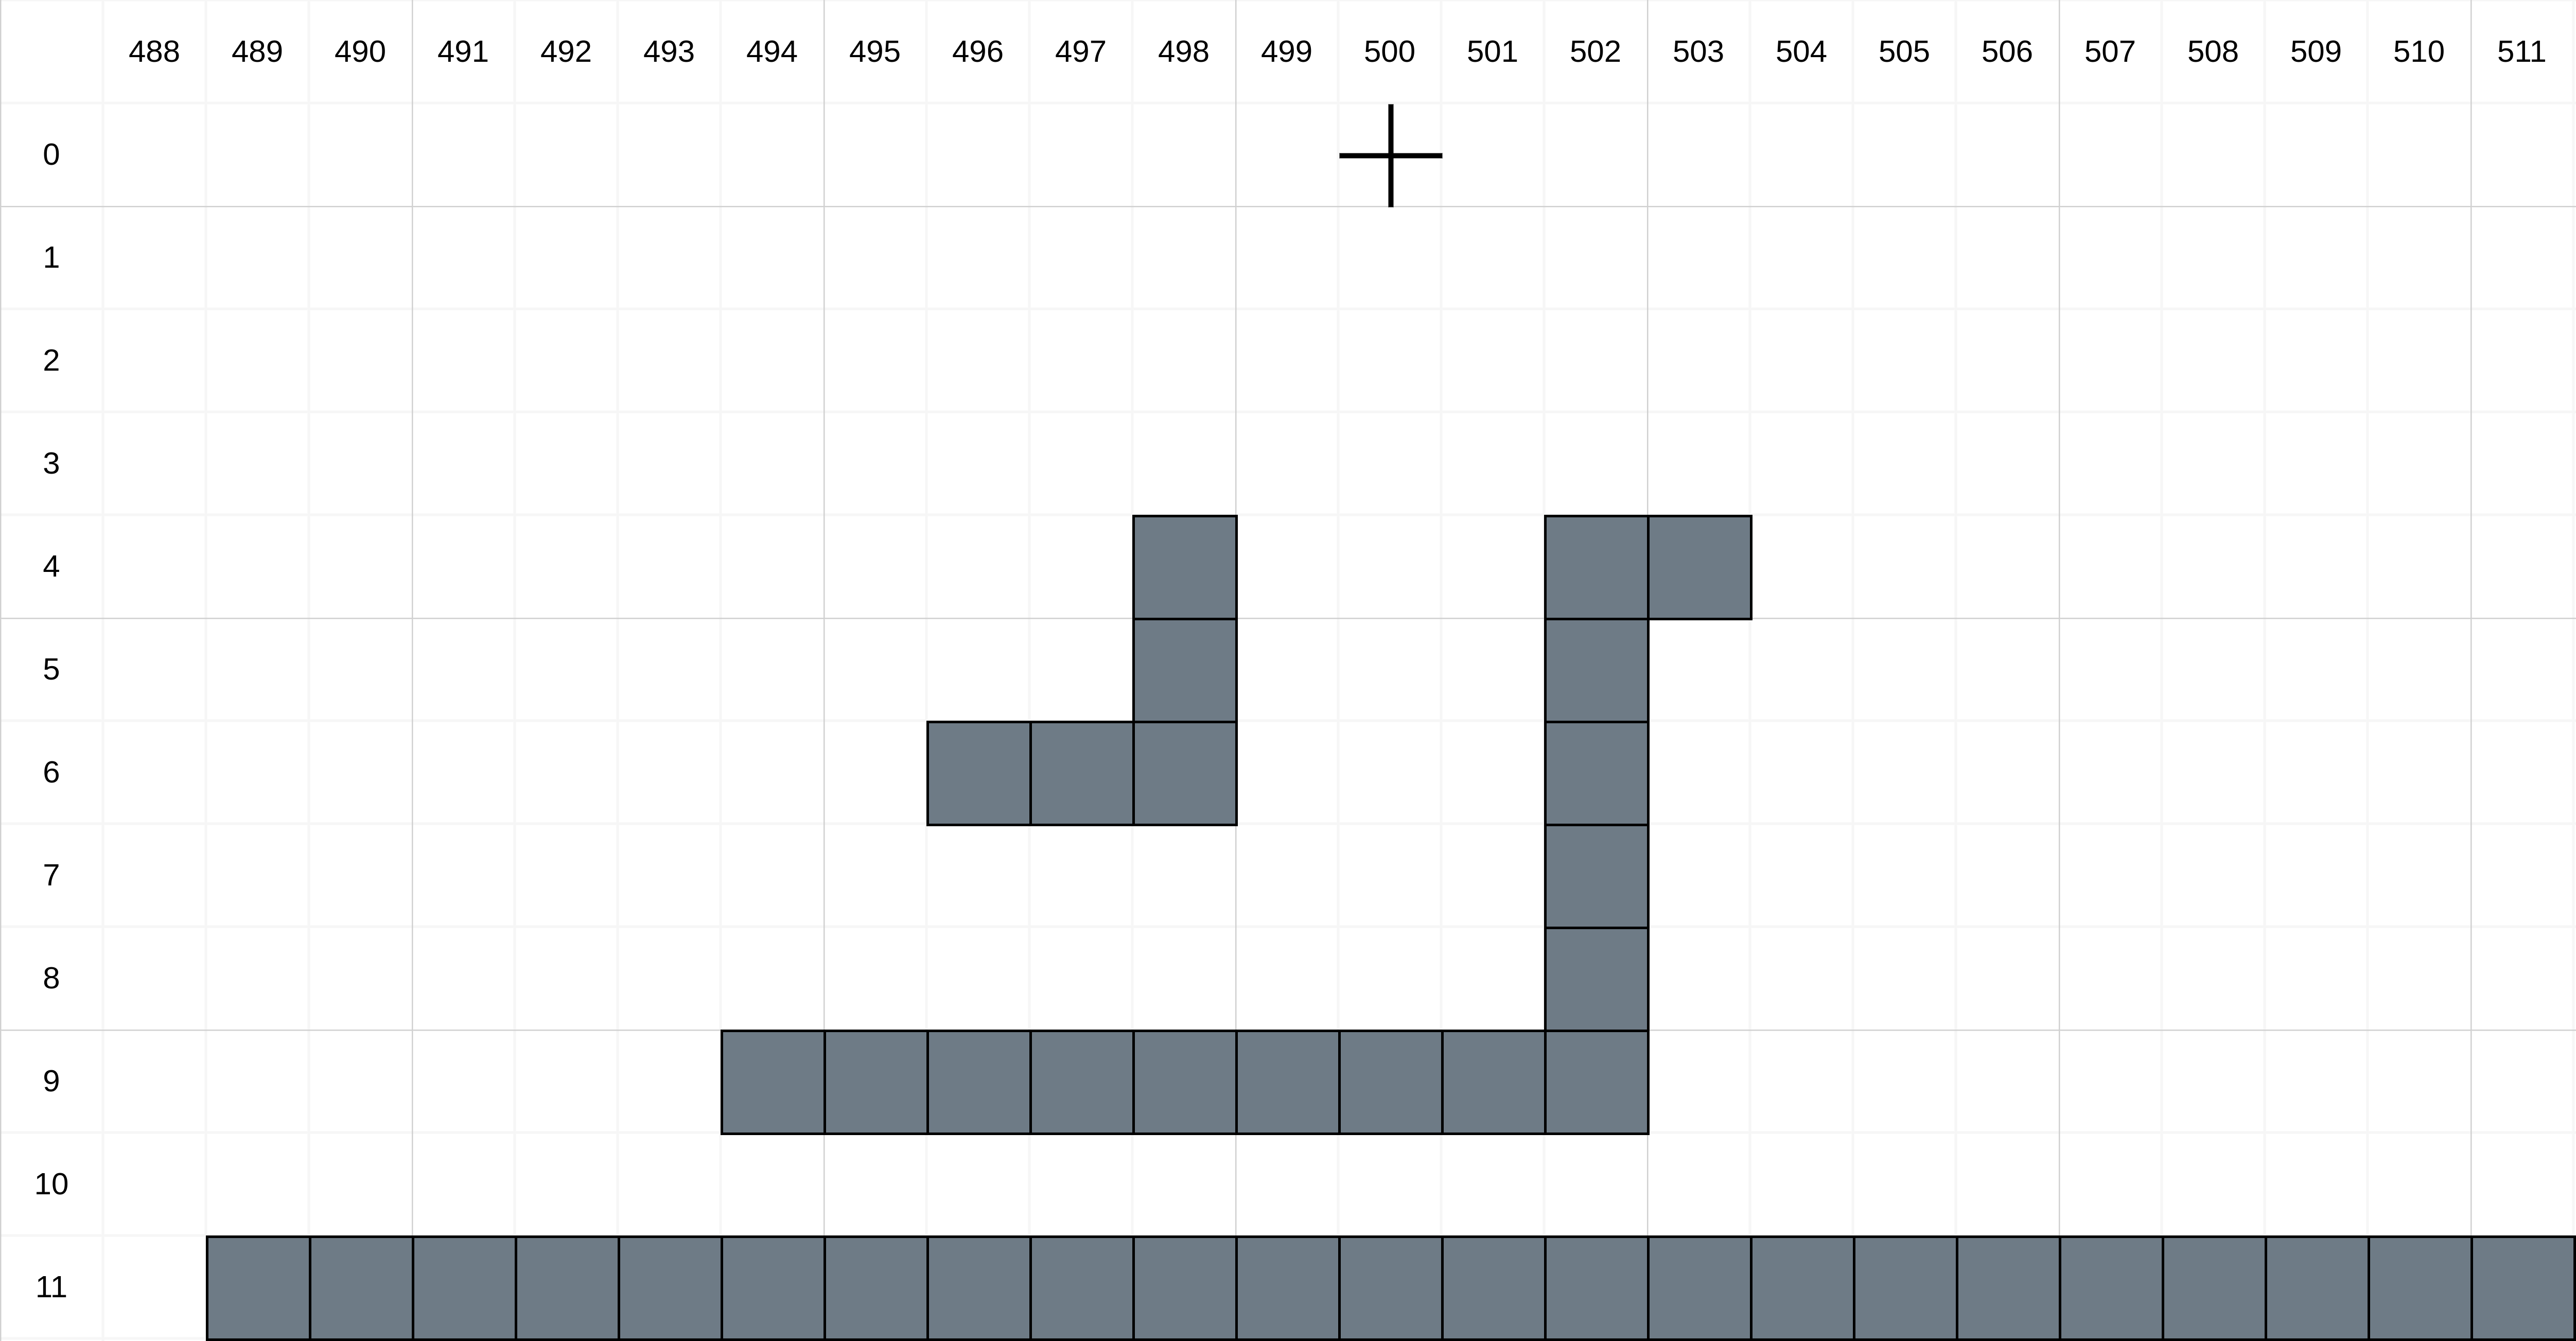
\includegraphics[width=0.8\textwidth]{Images/AoC22_14_Part_2_0_grid.png}
        \end{figure}
    \end{minipage}
\end{frame}

\section{Output Details}

\begin{frame}{Output Details}
    \begin{minipage}[c]{0.4\textwidth}
        \begin{figure}[H]
            \centering
            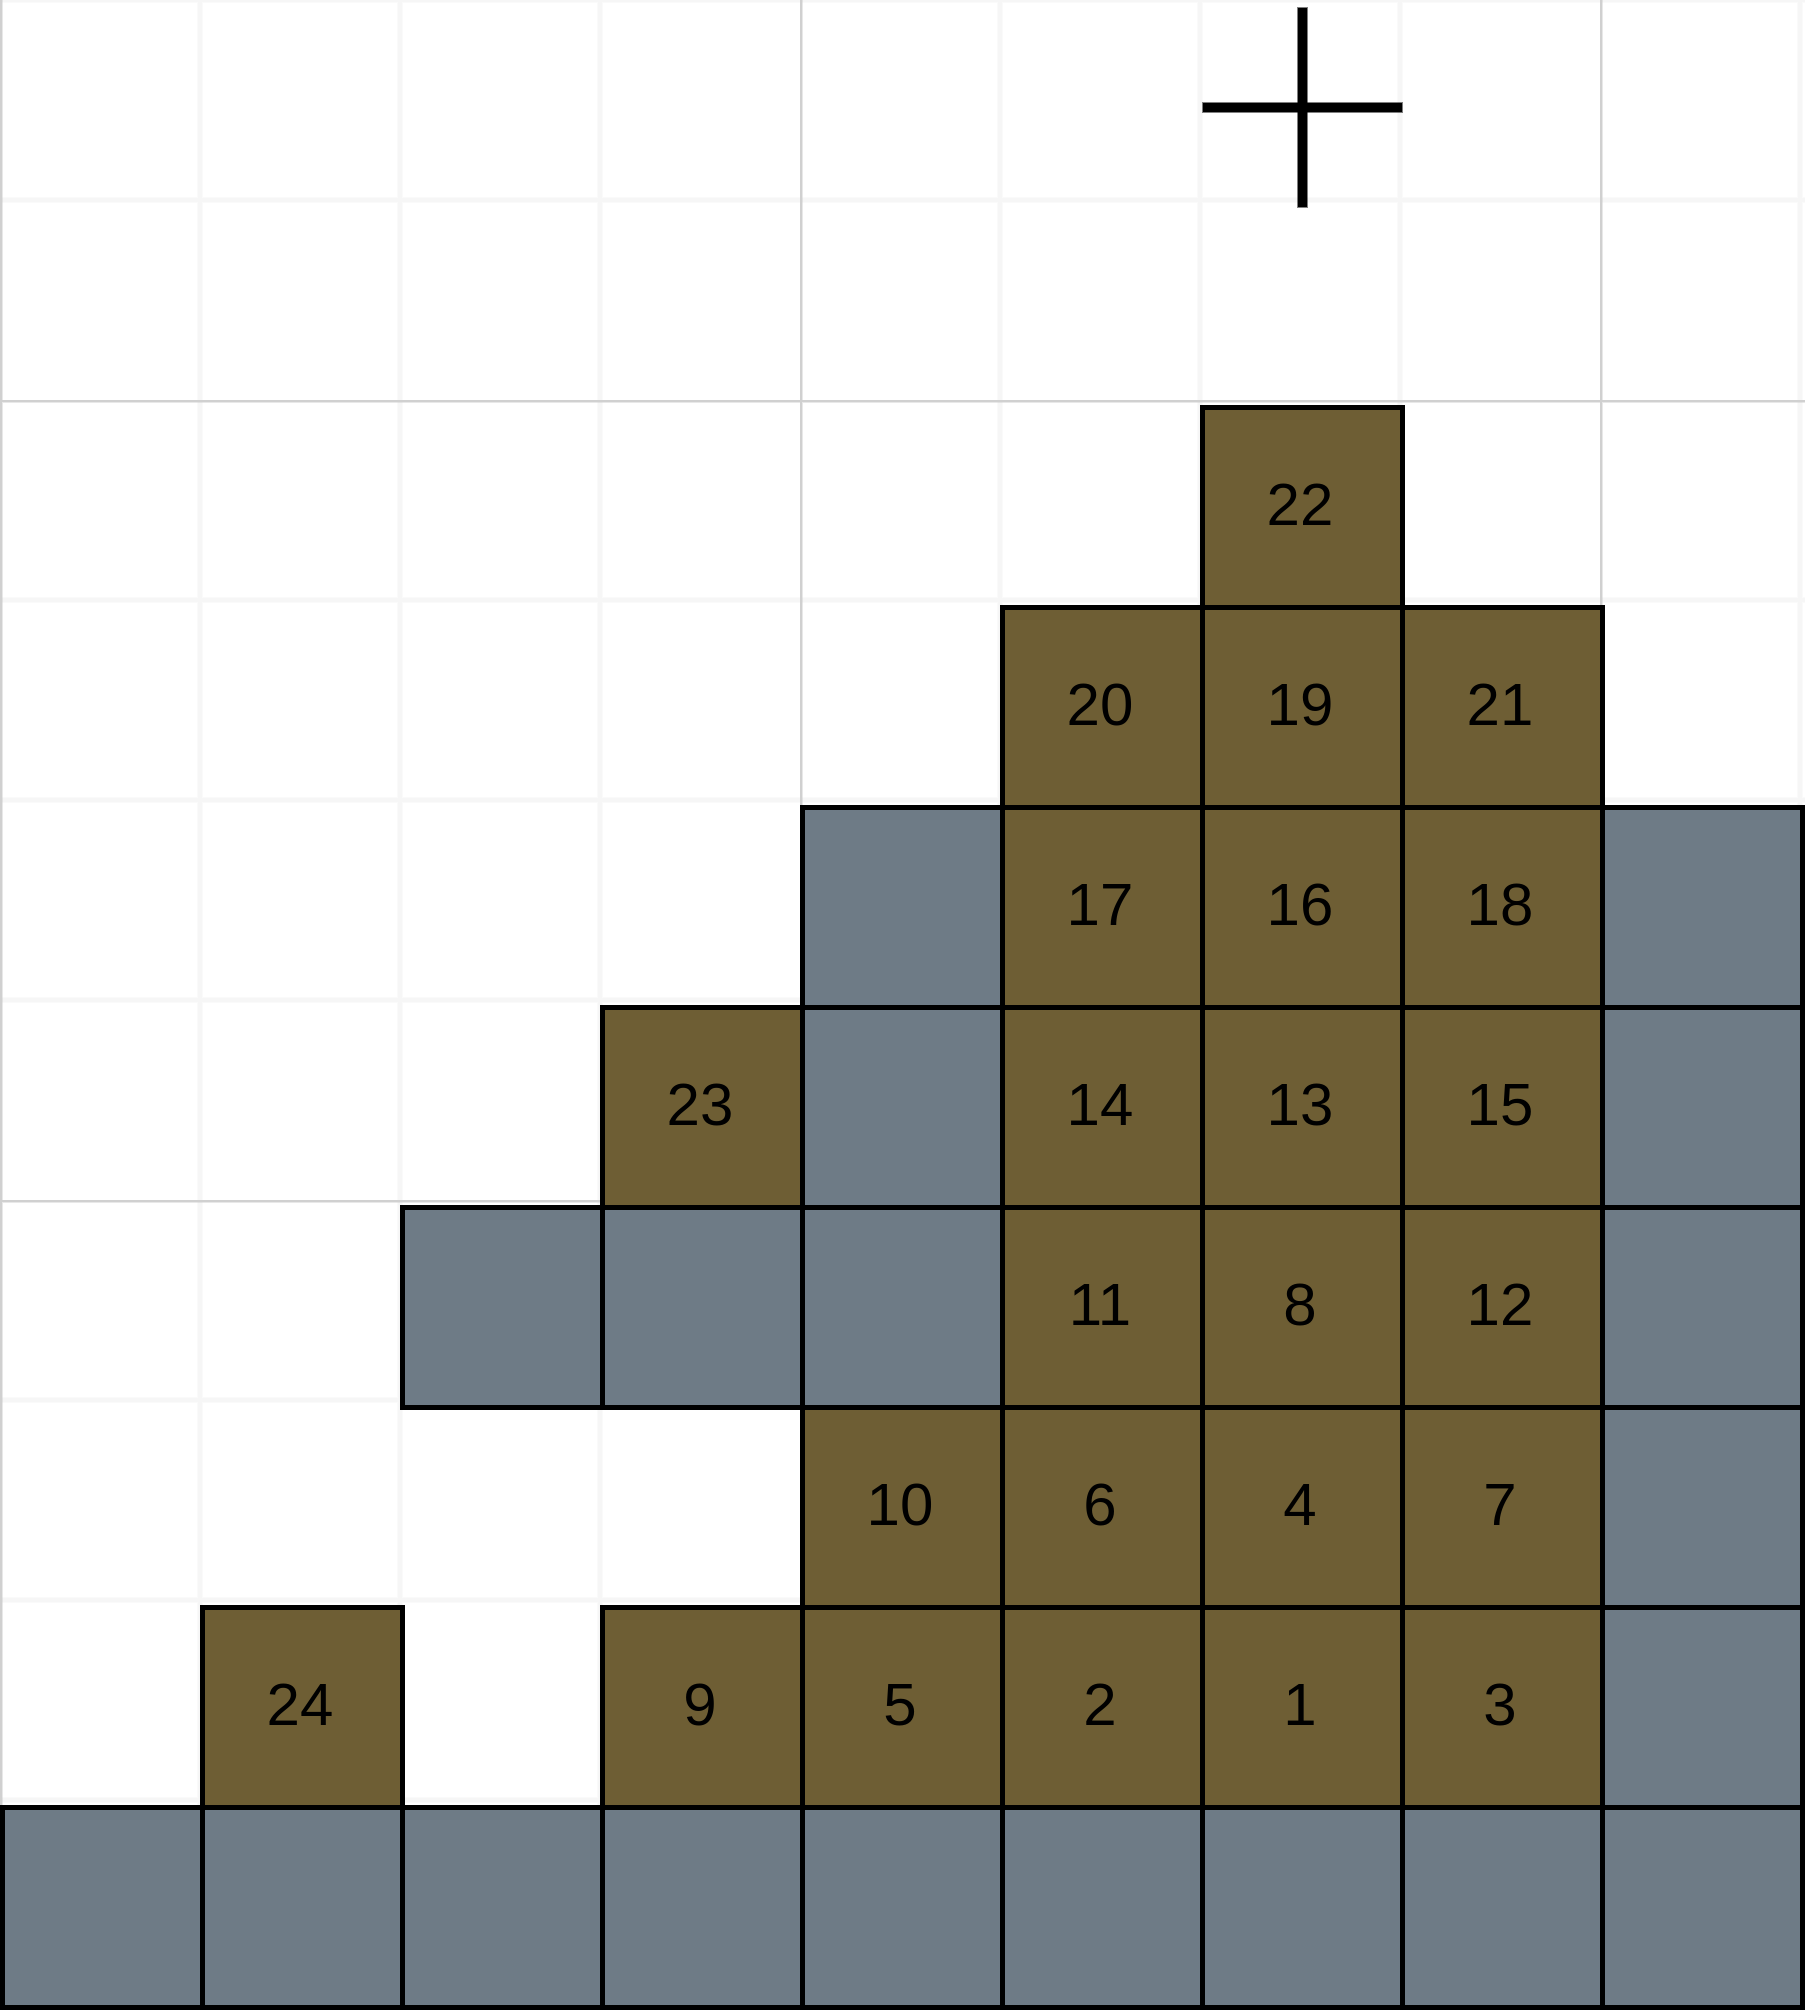
\includegraphics[width=0.565\textwidth]{Images/AoC22_14_solution_part_1.png}
        \end{figure}
    \end{minipage}%
    \begin{minipage}[c]{0.6\textwidth}
        \begin{figure}[H]
            \centering
            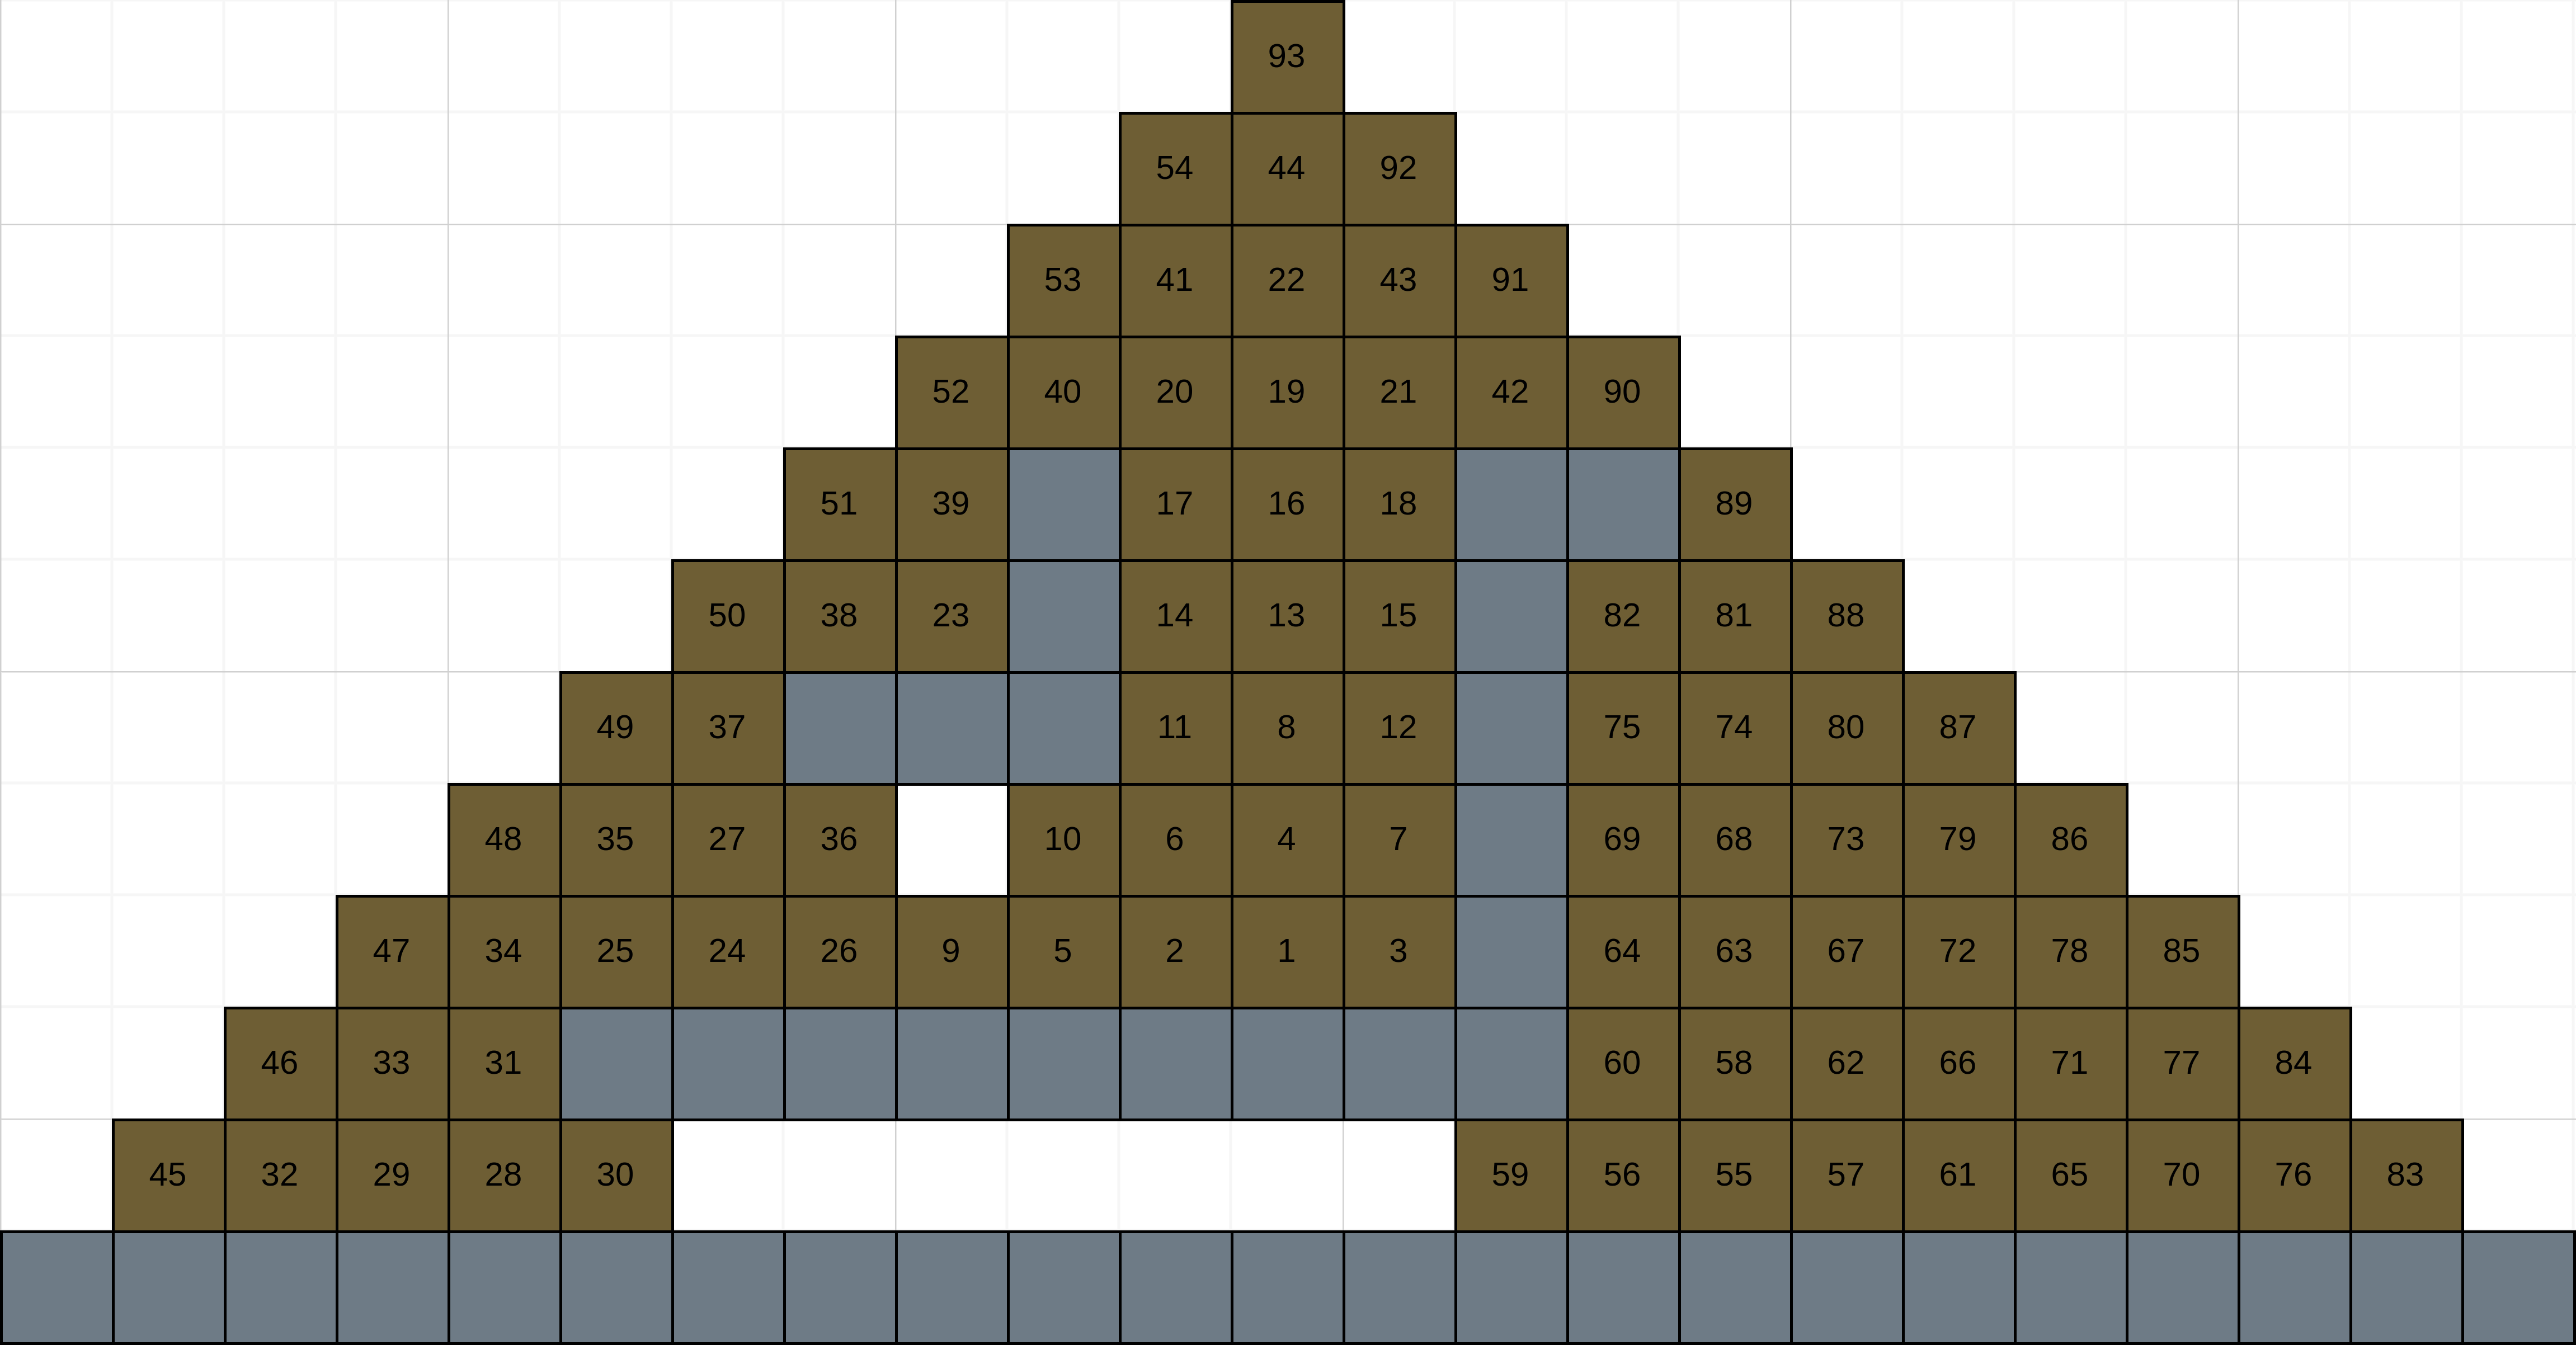
\includegraphics[width=0.8\textwidth]{Images/AoC22_14_solution_part_2.png}
        \end{figure}
    \end{minipage}
\end{frame}
\section{Solution Approach}

\begin{frame}{Solution Approach}
    \begin{figure}[H]
        \centering
        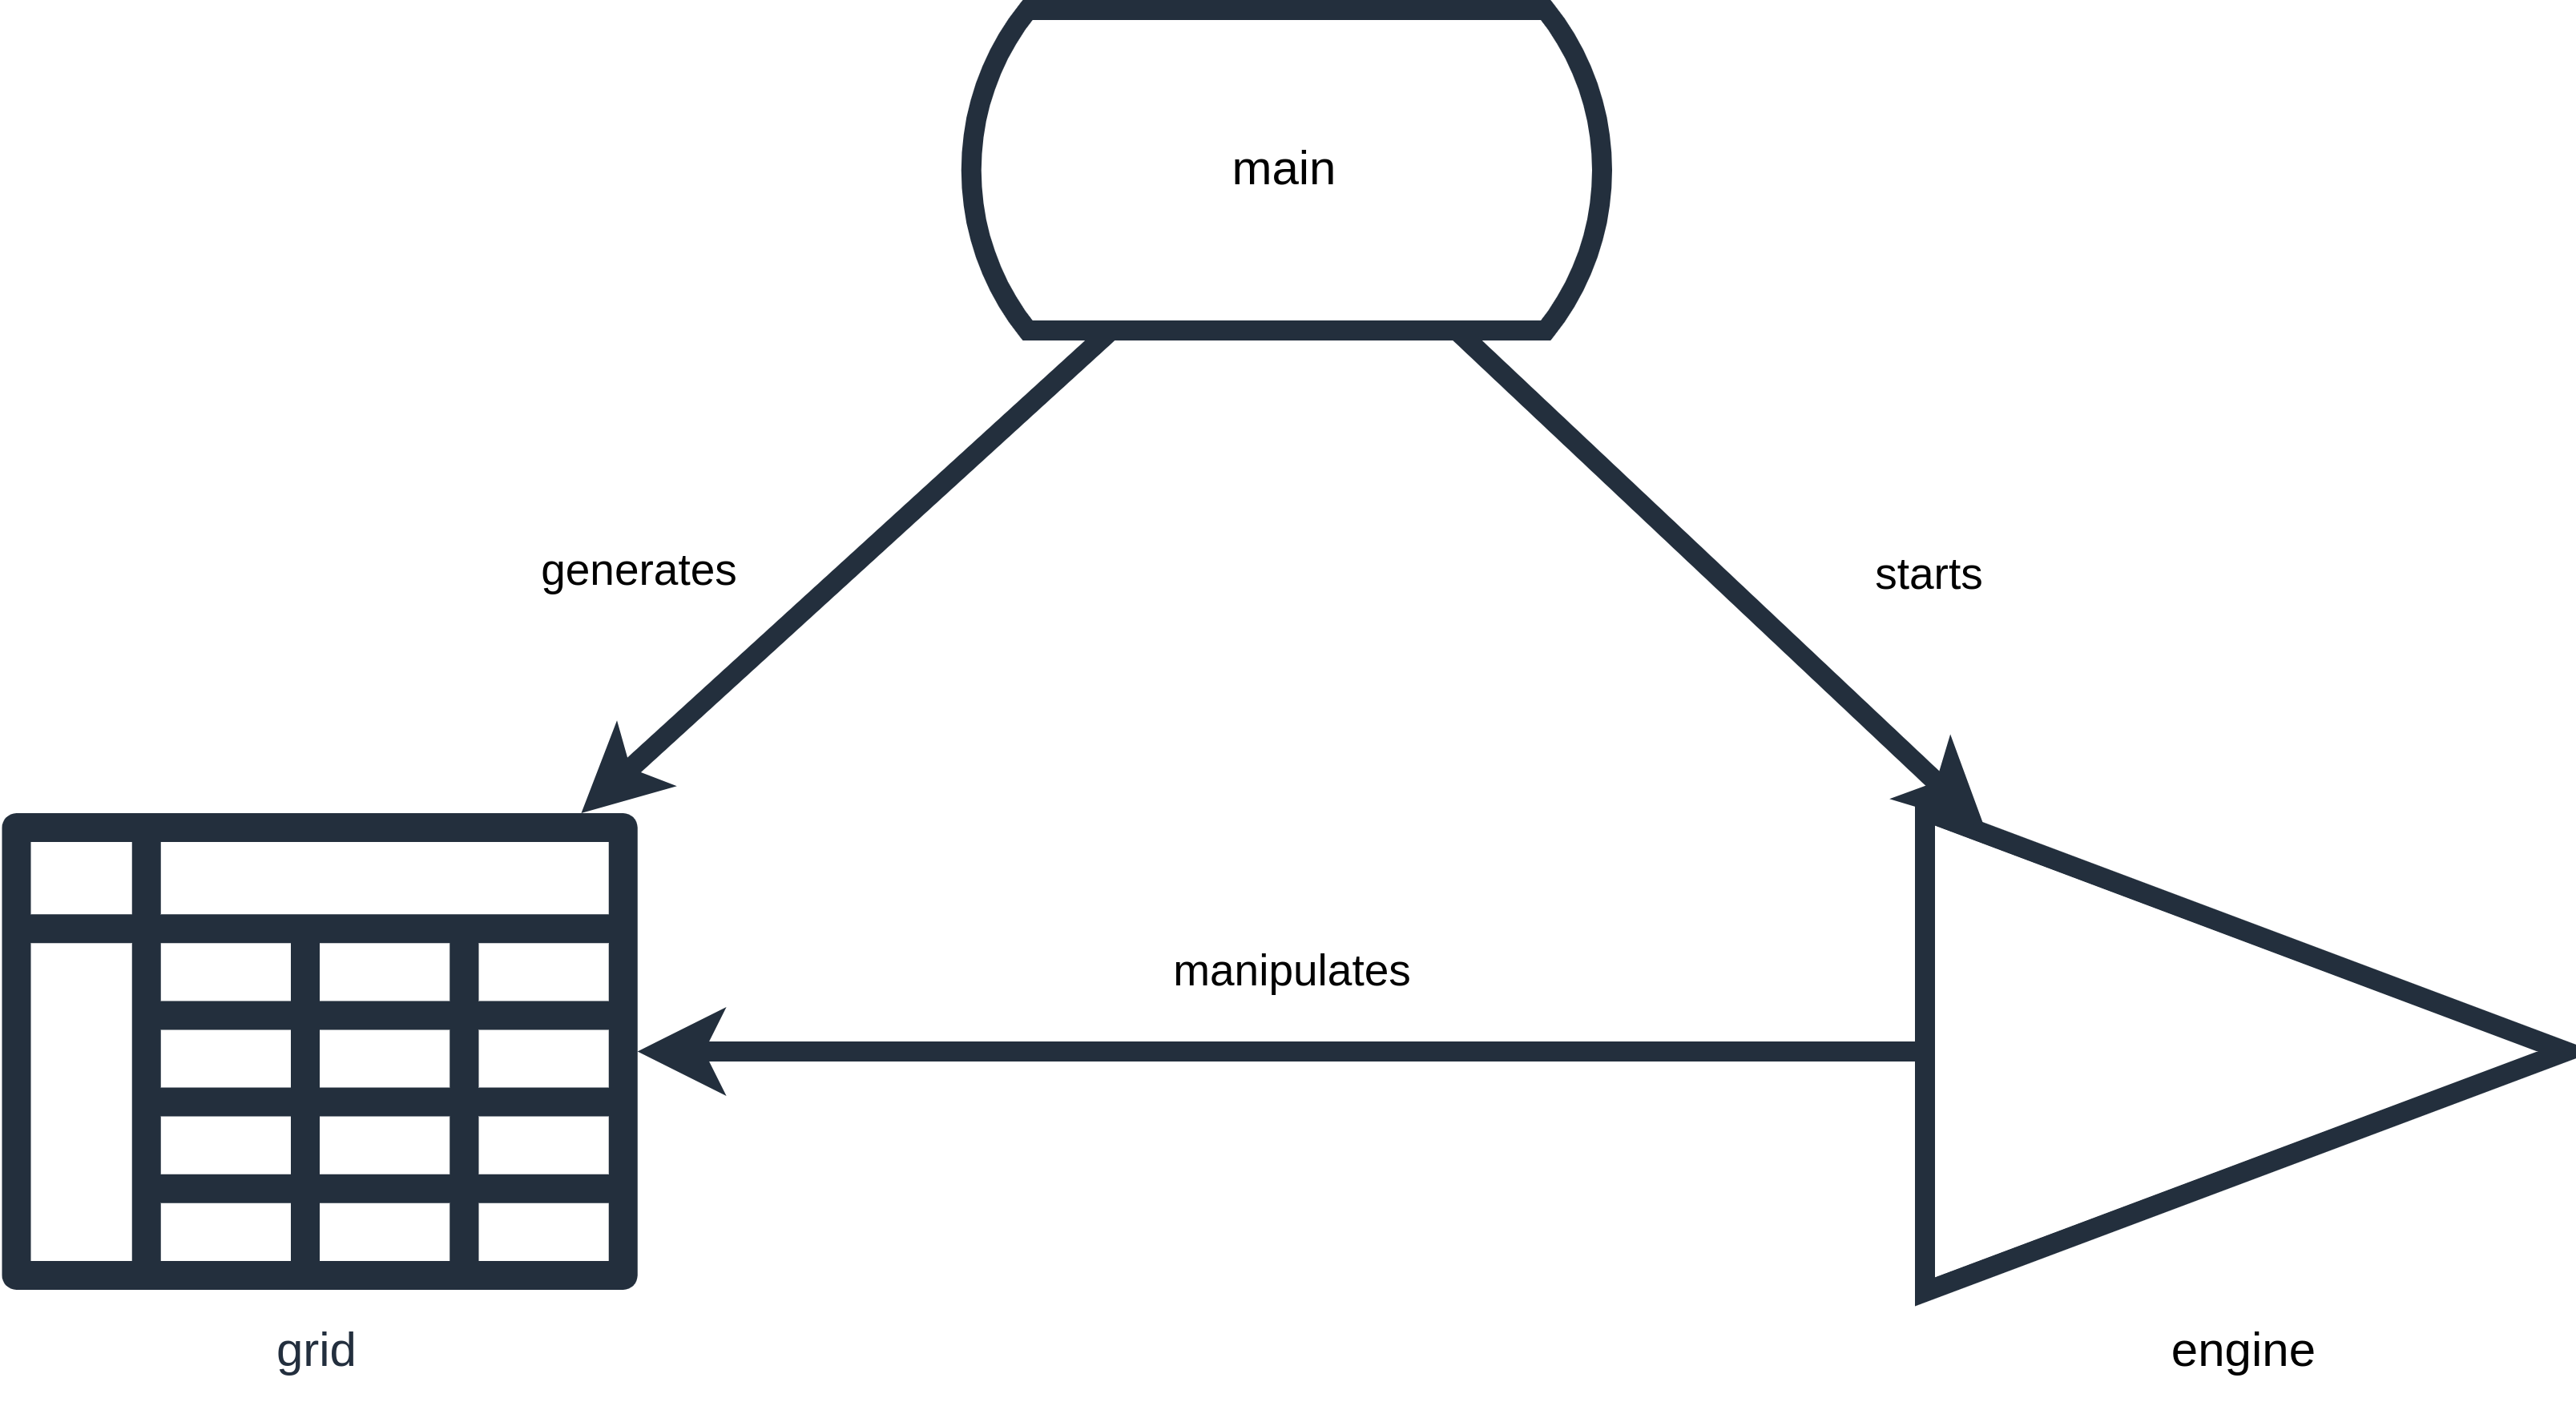
\includegraphics[width=0.8\textwidth]{Images/AoC22_14_high_level.png}
    \end{figure}
\end{frame}

% optionally also show grid generation
\section{Code Example}

\begin{frame}[fragile]{Code Example}
    \begin{minted}[bgcolor=codebg, linenos, fontsize=\scriptsize]{python}
num = 0
while True:
  sand = (500, 0)
  while True:
    if self.grid.is_air_at(Coordinate((sand[0], sand[1] + 1))):
      sand = (sand[0], sand[1] + 1)
    elif self.grid.is_air_at(Coordinate((sand[0] - 1, sand[1] + 1))):
      sand = (sand[0] - 1, sand[1] + 1)
    elif self.grid.is_air_at(Coordinate((sand[0] + 1, sand[1] + 1))):
      sand = (sand[0] + 1, sand[1] + 1)
    else:
      self.grid.add(Object((Material.solid_sand, Coordinate(sand))))
      break
    if sand[1] >= self.grid.get_last_row() + 1:
      if not part2:
        return num
      self.grid.add(Object((Material.solid_sand, Coordinate(sand))))
      break
  num += 1
  if sand == (500, 0):
    return num
    \end{minted}
\end{frame}

\section{Live Demo}

\begin{frame}{Live Demo}
\end{frame}

\section{Key Takeaways \& Outlook}

\begin{frame}{Key Takeaways \& Outlook}
    \begin{itemize}
        \only{\item<1-> rock structure is created using the input coordinates}
        \only{\item<2-> dynamically calculate the number of sand}
        \only{\item<3-> adjust grid to be optimized for memory or computational performance}
        \only{\item<4-> render falling sand}
    \end{itemize}
\end{frame}

\end{document}
